\section{Dimensionality reduction}


\newcommand{\motivationplot}[1]{
    \begin{tikzpicture}
        \begin{axis}[
            height=7cm,
            width=7cm,
            xlabel=$x_1$,
            ylabel=$x_2$,
            xmajorticks=false,
            ymajorticks=false
        ]
            \ifnum#1=0
                \addplot[
                    only marks,
                    blue,
                    opacity=0.5
                ] coordinates {
                    (-0.025, -0.056) %0
                    (-0.017, 0.026) %1
                    (-0.061, -0.061) %2
                    (0.01, -0.005) %3
                    (-0.073, -0.022) %4
                    (0.126, 0.126) %5
                    (0.132, 0.1) %6
                    (0.063, 0.121) %7
                    (0.099, 0.165) %8
                    (0.104, 0.079) %9
                    (0.16, -0.11) %10
                    (0.138, -0.157) %11
                    (0.153, -0.081) %12
                    (0.11, -0.1) %13
                    (0.122, -0.114) %14
                };
            \fi
            \ifnum#1=1
                \addplot[
                    only marks,
                    blue,
                    opacity=0.5
                ] (x, x + rand);
            \fi
        \end{axis}
    \end{tikzpicture}
}

\newsavebox{\motivationclusters}
\sbox{\motivationclusters}{
    \motivationplot{0}
}
\newsavebox{\motivationaxes}
\sbox{\motivationaxes}{
    \motivationplot{1}
}

\newsavebox{\overfitting}
\sbox{\overfitting}{
    \begin{tikzpicture}
        \begin{axis}[
            height=6cm,
            width=8cm,
            axis lines=left,
            xmajorticks=false,
            ymajorticks=false,
            ylabel=Loss,
            xlabel=$|p|$,
            ymin=-2,
            xmin=-1,
            xmax=3
        ]
            \addplot[thick, red, domain=-1:3, samples=100] (x, x^2);
        \end{axis}
    \end{tikzpicture}
}

\newcommand{\predictorplot}[1]{
    \nextgroupplot[]
        \addplot[
            only marks,
            blue,
            opacity=0.5
        ] table [
            col sep=comma,
            x=#1,
            y=mpg
        ] {data/Auto.csv};
}

\newcommand{\correlationplot}[1]{
    \begin{tikzpicture}
        \begin{groupplot}[
            group style={group size=2 by 3}
        ]
            \predictorplot{cylinders}
        \end{groupplot}
    \end{tikzpicture}
}

\newsavebox{\correlationpredictors}
\sbox{\correlationpredictors}{
    \correlationplot{0}
}

\begin{frame}{Dimensionality reduction: Motivation}
    \begin{tikzpicture}
        \node[] at (-5.25, 3.5) {};
        \node[] at (-5.25, -3.5) {};

        \visible<1>{
            \node[] at (0, 0) {
                \usebox{\motivationclusters}
            };
        }
        \visible<2>{
            \node[] at (0, 0) {
                \usebox{\motivationaxes}
            };
        }
        \visible<3>{
            \node[draw=black, inner sep=0pt, anchor=west] (test) at (-4, 0) {
                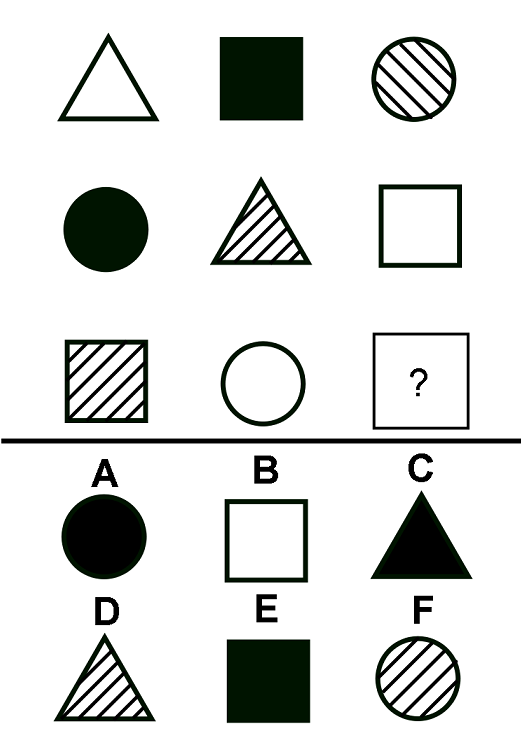
\includegraphics[height=4cm]{data/iqtest.png}
            };
            \node[draw=black, dashed, anchor=east, align=center] (iq) at (4, 0) {
                Intelligence\\quotient
            };
            \draw[-stealth, line width=5pt, gray] (test) -- (iq);
        }
        \visible<4>{
            \node[] at (0, 0) {
                \usebox{\overfitting}
            };
        }
        \visible<5>{
            \node[] at (0, 0) {
                \usebox{\correlationpredictors}
            };
        }
    \end{tikzpicture}
\end{frame}
